% AgentCore Strategic Assessment: Full Python Port and Bedrock-Native Architecture
% Strategic Planning Document - Q3/Q4 2026
\documentclass[11pt,letterpaper]{article}

\usepackage[utf8]{inputenc}
\usepackage[margin=1in]{geometry}
\usepackage{amsmath,amssymb}
\usepackage{listings}
\usepackage{xcolor}
\usepackage{hyperref}
\usepackage{booktabs}
\usepackage{graphicx}
\usepackage{tikz}
\usepackage{fancyhdr}
\usepackage{enumitem}
\usepackage{multirow}
\usepackage{tabularx}
\usepackage{longtable}
\usepackage{float}

\usetikzlibrary{shapes.geometric, arrows.meta, positioning, fit, backgrounds, calc}

\definecolor{awsorange}{HTML}{FF9900}
\definecolor{awsblue}{HTML}{232F3E}
\definecolor{noaablue}{HTML}{003087}
\definecolor{strandspurple}{HTML}{7B2FBE}
\definecolor{pythonblue}{HTML}{3776AB}
\definecolor{nodejsgreen}{HTML}{339933}
\definecolor{cedargreen}{HTML}{2E7D32}

\hypersetup{
    colorlinks=true,
    linkcolor=noaablue,
    citecolor=noaablue,
    urlcolor=awsorange,
    pdftitle={AgentCore Strategic Assessment},
    pdfauthor={NOAA MDC Global Workflow MCP Team}
}

\lstset{
    basicstyle=\ttfamily\footnotesize,
    breaklines=true,
    frame=single,
    captionpos=b,
    numbers=left,
    numberstyle=\tiny\color{gray},
    keywordstyle=\color{blue},
    commentstyle=\color{green!60!black},
    stringstyle=\color{red},
    backgroundcolor=\color{gray!5},
    showstringspaces=false
}

\pagestyle{fancy}
\fancyhf{}
\rhead{AgentCore Strategic Assessment}
\lhead{NOAA MDC --- Q3/Q4 2026 Planning}
\cfoot{\thepage}

\title{\textbf{Amazon Bedrock AgentCore} \\
       \textbf{Strategic Assessment for MDC MCP/RAG Platform} \\[0.5em]
       \large Full Python Port vs.\ Container Deployment: \\
       \large Capabilities, Trade-offs, and Quarterly Roadmap}

\author{
    Terrence McGuinness \\
    Modeling Development Center \\
    National Weather Service, NOAA \\
    \texttt{Terry.McGuinness@noaa.gov}
}

\date{April 22, 2026}

\begin{document}

\maketitle

\begin{abstract}
This document assesses the strategic options for integrating the MDC
MCP/RAG Server---a 51-tool AI development platform for NOAA's Global
Forecast System---with Amazon Bedrock AgentCore. We evaluate two paths:
(A)~container deployment of the existing Node.js server to AgentCore
Runtime, and (B)~a full port to Python using the Strands Agents SDK
with native AgentCore primitives (Memory, Gateway, Policy, Observability,
Evaluations, Browser, Code Interpreter, and Registry). Path~A delivers
immediate production deployment with minimal effort. Path~B unlocks
autonomous multi-agent orchestration, persistent cross-session memory,
Cedar-based policy enforcement, OpenTelemetry observability, and
integration with the broader Bedrock foundation model ecosystem. We
present a phased quarterly roadmap that begins with container deployment
(Q3~2026) and progressively adopts AgentCore primitives, culminating in
a fully Bedrock-native agentic platform (Q4~2026--Q1~2027).

\textbf{Keywords:} AgentCore, Bedrock, Strands Agents, MCP, Python,
Multi-Agent Orchestration, Memory, Gateway, Cedar Policy, OpenTelemetry
\end{abstract}

\tableofcontents
\newpage

%===============================================================================
\section{Executive Summary}
%===============================================================================

The MDC MCP/RAG Server has evolved through 52 development phases into a
51-tool platform serving AI-assisted development of the Global Forecast
System. The current architecture runs on Node.js with JavaScript across
9 modules, backed by Amazon OpenSearch (vector search) and Amazon Neptune
(graph queries). It works---45/45 tools pass validation, 6/6 parity
benchmarks meet targets.

Amazon Bedrock AgentCore, generally available since October 2025, offers
9 modular services purpose-built for agentic AI workloads. Adopting
AgentCore is not just a deployment decision---it is an architectural
inflection point that determines whether the platform remains a
\textit{tool server} or evolves into an \textit{autonomous agent
ecosystem}.

\subsection{The Two Paths}

\begin{table}[H]
\centering
\footnotesize
\begin{tabular}{@{}p{3cm}p{5.5cm}p{5.5cm}@{}}
\toprule
& \textbf{Path A: Container Deploy} & \textbf{Path B: Full Python Port} \\
\midrule
\textbf{Effort} & 1--2 weeks & 3--4 months \\
\textbf{Language} & Keep Node.js/JavaScript & Port to Python (Strands SDK) \\
\textbf{AgentCore Services} & Runtime only & All 9 services \\
\textbf{What It Unlocks} & Managed hosting, auto-scaling, CloudFormation & Multi-agent orchestration, memory, policy, observability, evaluations, browser, code interpreter, registry \\
\textbf{Risk} & Low (no code changes) & Medium (full rewrite) \\
\textbf{Strategic Value} & Tactical (ship it) & Transformational \\
\bottomrule
\end{tabular}
\caption{Path comparison summary.}
\end{table}

\subsection{Recommendation}

Execute both paths sequentially: Path~A in Q3~2026 for immediate
production deployment, then Path~B as a Q4~2026--Q1~2027 initiative
that progressively ports modules to Python while the Node.js server
continues serving production traffic.

%===============================================================================
\section{Current Architecture Baseline}
%===============================================================================

\subsection{System Inventory}

\begin{table}[H]
\centering
\footnotesize
\begin{tabular}{@{}llr@{}}
\toprule
\textbf{Component} & \textbf{Technology} & \textbf{Scale} \\
\midrule
MCP Server & Node.js 20, JavaScript (ES modules) & 51 tools, 9 modules \\
Vector Search & Amazon OpenSearch (k-NN) & 85,921 docs, 768/1024-dim \\
Graph Database & Amazon Neptune (openCypher) & 59,759 nodes, 2.6M rels \\
Embedding Models & MPNet-768 (local), Titan-1024, Nova (Bedrock) & 6 profiles \\
HTTP Transport & \texttt{mcp-http-server.js} (Streamable HTTP) & Port 3000 \\
SDD Framework & 53 workflows, 32 sessions & JSONL persistence \\
\bottomrule
\end{tabular}
\caption{Current system inventory on \texttt{develop\_aws} branch.}
\end{table}

\subsection{Code Volume}

\begin{table}[H]
\centering
\footnotesize
\begin{tabular}{@{}llr@{}}
\toprule
\textbf{Module} & \textbf{Primary Files} & \textbf{Approx.\ Lines} \\
\midrule
UnifiedMCPServer & \texttt{UnifiedMCPServer.js} & 1,300 \\
CodeAnalysisTools & \texttt{CodeAnalysisTools.js} & 1,300 \\
GraphRAGTools & \texttt{GraphRAGTools.js} & 925 \\
OperationalTools & \texttt{OperationalTools.js} & 894 \\
SemanticSearchTools & \texttt{SemanticSearchTools.js} & $\sim$800 \\
EE2ComplianceTools & \texttt{EE2ComplianceTools.js} & $\sim$600 \\
SDDWorkflowTools & \texttt{SDDWorkflowTools.js} & $\sim$700 \\
WorkflowInfoTools & \texttt{WorkflowInfoTools.js} & $\sim$400 \\
NeptuneAdapter & \texttt{NeptuneAdapter.js} & $\sim$650 \\
OpenSearchAdapter & \texttt{OpenSearchAdapter.js} & $\sim$500 \\
GGSR Traversal & \texttt{GGSRTraversalPrototypes.js} & $\sim$600 \\
GraphGuidedRetrieval & \texttt{GraphGuidedRetrieval.js} & $\sim$400 \\
Ingestion Scripts (Python) & 14 scripts & $\sim$4,000 \\
\midrule
\textbf{Total JavaScript} & & $\sim$9,000 \\
\textbf{Total Python (ingestion)} & & $\sim$4,000 \\
\bottomrule
\end{tabular}
\caption{Code volume by module. The ingestion pipeline is already Python.}
\end{table}


%===============================================================================
\section{AgentCore Platform: 9 Services Deep Dive}
%===============================================================================

\begin{figure}[H]
\centering
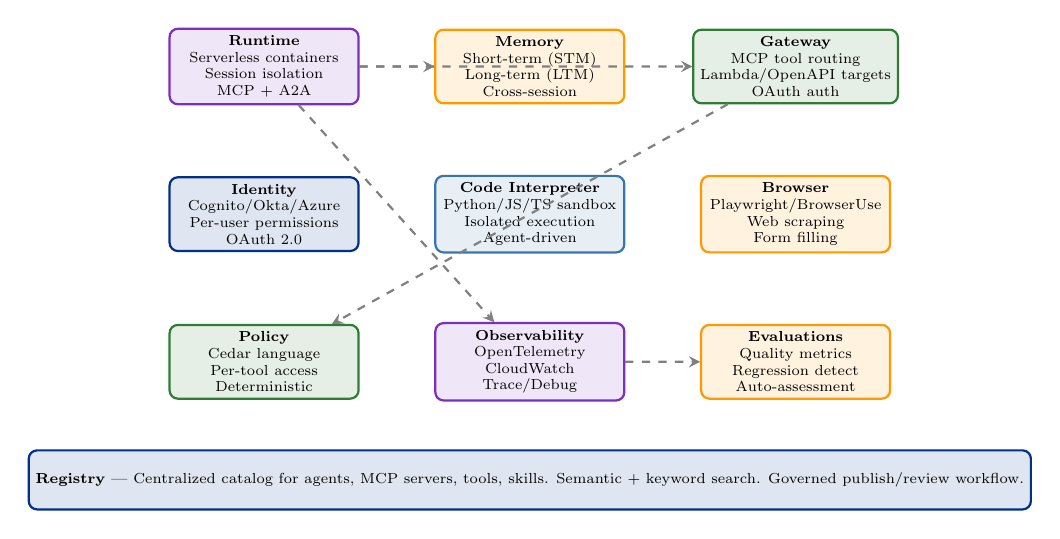
\begin{tikzpicture}[
    scale=0.75,
    every node/.style={transform shape},
    service/.style={rectangle, draw=#1, fill=#1!12, minimum width=3.2cm,
                   minimum height=1cm, font=\scriptsize, align=center,
                   rounded corners=3pt, thick},
    service/.default=awsorange,
    arrow/.style={->, thick, >=stealth}
]

% Core services
\node[service=strandspurple] at (0,6) (runtime) {\textbf{Runtime}\\Serverless containers\\Session isolation\\MCP + A2A};
\node[service=awsorange] at (4.5,6) (memory) {\textbf{Memory}\\Short-term (STM)\\Long-term (LTM)\\Cross-session};
\node[service=cedargreen] at (9,6) (gateway) {\textbf{Gateway}\\MCP tool routing\\Lambda/OpenAPI targets\\OAuth auth};

\node[service=noaablue] at (0,3.5) (identity) {\textbf{Identity}\\Cognito/Okta/Azure\\Per-user permissions\\OAuth 2.0};
\node[service=pythonblue] at (4.5,3.5) (code) {\textbf{Code Interpreter}\\Python/JS/TS sandbox\\Isolated execution\\Agent-driven};
\node[service=awsorange] at (9,3.5) (browser) {\textbf{Browser}\\Playwright/BrowserUse\\Web scraping\\Form filling};

\node[service=cedargreen] at (0,1) (policy) {\textbf{Policy}\\Cedar language\\Per-tool access\\Deterministic};
\node[service=strandspurple] at (4.5,1) (observe) {\textbf{Observability}\\OpenTelemetry\\CloudWatch\\Trace/Debug};
\node[service=awsorange] at (9,1) (eval) {\textbf{Evaluations}\\Quality metrics\\Regression detect\\Auto-assessment};

% Registry at bottom
\node[service=noaablue, minimum width=12.5cm] at (4.5,-1) (registry) {\textbf{Registry} --- Centralized catalog for agents, MCP servers, tools, skills. Semantic + keyword search. Governed publish/review workflow.};

% Connections
\draw[arrow, gray, dashed] (runtime) -- (memory);
\draw[arrow, gray, dashed] (runtime) -- (gateway);
\draw[arrow, gray, dashed] (gateway) -- (policy);
\draw[arrow, gray, dashed] (runtime) -- (observe);
\draw[arrow, gray, dashed] (observe) -- (eval);

\end{tikzpicture}
\caption{AgentCore's 9 modular services. Each can be adopted independently.}
\label{fig:agentcore-services}
\end{figure}

\subsection{Runtime}

Serverless container hosting purpose-built for AI agents and MCP servers.
Expects HTTP at \texttt{0.0.0.0:8000/mcp}. Supports stateless and stateful
Streamable HTTP. Session isolation via microVMs. Fast cold starts.
CloudFormation-managed via \texttt{agentcore deploy}.

\textbf{Current gap}: Our server runs on a manually started process
(\texttt{start-aws-mcp.sh}) with a security group hack for port 3000.

\textbf{Path A value}: Immediate---change port to 8000, containerize, deploy.

\subsection{Memory}

Managed short-term memory (conversation history within a session) and
long-term memory (insights extracted across sessions). Agents can share
memory stores. Integrates with Strands, LangGraph, LangChain, LlamaIndex.

\textbf{Current gap}: SDD session state persists to \texttt{history.jsonl}
on local disk. No cross-session learning. No shared memory between agents.

\textbf{Path B value}: SDD sessions, query feedback, user preferences,
and code analysis context could persist in AgentCore Memory, enabling
agents to learn from past interactions and share knowledge.

\subsection{Gateway}

Converts APIs, Lambda functions, and MCP servers into unified tool
endpoints. Handles OAuth authentication, routing, and rate limiting.
Supports multiple targets per gateway.

\textbf{Current gap}: Docker MCP Gateway (legacy) or Private API Gateway
(AWS) handle routing. No per-tool auth or rate limiting.

\textbf{Path B value}: Publish our 51 tools as Gateway targets with
per-tool Cedar policies. External teams could consume specific tools
(e.g., EE2 compliance checking) without access to the full server.

\subsection{Identity}

Agent identity management compatible with Cognito, Okta, Azure AD, Auth0.
Per-user agent permissions. OAuth 2.0 flows.

\textbf{Current gap}: Bearer token auth (single shared token) or VPC
resource policy (no per-user identity).

\textbf{Path B value}: Per-developer tool access. Audit trail of who
used which tool. Integration with NOAA's identity provider.

\subsection{Code Interpreter}

Isolated sandbox for agents to execute Python, JavaScript, and TypeScript
code. Agents can write and run code to solve complex tasks.

\textbf{Current gap}: Ingestion scripts run manually on EC2. No
agent-driven code execution.

\textbf{Path B value}: Agents could autonomously run ingestion scripts,
benchmarks, or data analysis. A Strands agent could decide ``the
community summaries are stale'' and trigger re-ingestion without human
intervention.

\subsection{Browser}

Cloud-based browser runtime for web interaction. Playwright and BrowserUse
support. Form filling, navigation, data extraction.

\textbf{Current gap}: Documentation crawling uses \texttt{ingestion\_base.py}
with \texttt{requests} + BeautifulSoup. Rate-limited sites (MOM6, CICE)
require manual retry.

\textbf{Path B value}: Agent-driven documentation crawling that handles
JavaScript-rendered pages, CAPTCHAs, and rate limiting automatically.
Could replace the entire documentation ingestion pipeline.

\subsection{Policy (Cedar)}

Deterministic access control using Cedar, AWS's open-source policy
language. Policies are human-readable, analyzable, and schema-validated.
Intercepts every tool call before execution.

\textbf{Current gap}: No per-tool access control. All authenticated
users can call all 51 tools.

\textbf{Path B value}: Role-based tool access. Example Cedar policy:

\begin{lstlisting}[caption={Cedar policy restricting EE2 compliance tools to auditors.}]
permit(
  principal is AgentCore::OAuthUser,
  action == AgentCore::Action::"CallTool",
  resource is AgentCore::Gateway::"mdc-mcp-rag"
) when {
  resource.toolName in [
    "analyze_ee2_compliance",
    "scan_repository_compliance",
    "generate_compliance_report"
  ] && principal.groups.contains("ee2-auditors")
};
\end{lstlisting}

\subsection{Observability}

OpenTelemetry-compatible tracing, debugging, and performance monitoring.
Integrates with CloudWatch, Dynatrace, Elastic, and Datadog. Traces
every agent step: LLM calls, tool invocations, memory retrievals.

\textbf{Current gap}: \texttt{health\_history.jsonl} with manual drift
detection. No distributed tracing. No per-tool latency breakdown.

\textbf{Path B value}: Full OpenTelemetry traces for every MCP tool
call. Automatic anomaly detection. Integration with CloudWatch dashboards.
Replaces our custom \texttt{get\_health\_trend} and \texttt{mcp\_health\_check}
tools with managed infrastructure.

\subsection{Evaluations}

Automated agent quality assessment. Measures task execution, edge case
handling, and output reliability. Integrates with CloudWatch for
continuous monitoring.

\textbf{Current gap}: \texttt{benchmark\_runner.py} with 24 ground-truth
queries. Manual execution. Results stored in S3.

\textbf{Path B value}: Continuous automated quality monitoring in
production. Regression detection on every deployment. Replaces our
custom \texttt{get\_quality\_metrics} tool.

\subsection{Registry}

Centralized catalog for discovering and managing agents, MCP servers,
tools, and skills. Semantic + keyword search. Governed publish/review
workflow.

\textbf{Current gap}: Tools are discoverable only via \texttt{tools/list}
MCP call. No organizational catalog.

\textbf{Path B value}: Publish the MDC MCP tools to an organizational
registry. Other NOAA teams could discover and consume our EE2 compliance,
code analysis, or operational guidance tools.

%===============================================================================
\section{Path A: Container Deployment (Q3 2026)}
%===============================================================================

\subsection{Scope}

Deploy the existing Node.js MCP server to AgentCore Runtime with zero
code changes to the 51 tools. Estimated effort: 1--2 weeks.

\subsection{Implementation Steps}

\begin{enumerate}[noitemsep]
    \item Modify \texttt{mcp-http-server.js}: change port from 3000 to 8000
    \item Update Dockerfile: set \texttt{EXPOSE 8000}, add
          \texttt{CMD ["node", "src/mcp-http-server.js", "8000", "full"]}
    \item Install AgentCore CLI: \texttt{npm install -g @aws/agentcore}
    \item Create project: \texttt{agentcore create --protocol MCP}
    \item Configure: point entrypoint to our Dockerfile
    \item Deploy: \texttt{agentcore deploy}
    \item Update Kiro MCP config with AgentCore endpoint URL
    \item Remove port 3000 security group rule and dev bridge
\end{enumerate}

\subsection{What Path A Delivers}

\begin{itemize}[noitemsep]
    \item CloudFormation-managed deployment (IaC)
    \item Auto-scaling and session isolation
    \item OAuth authentication via Cognito
    \item No more manual \texttt{start-aws-mcp.sh}
    \item No more security group hacks
\end{itemize}

\subsection{What Path A Does NOT Deliver}

\begin{itemize}[noitemsep]
    \item No multi-agent orchestration
    \item No persistent memory across sessions
    \item No Cedar policy enforcement
    \item No OpenTelemetry observability
    \item No automated evaluations
    \item No agent-driven code execution or browser automation
\end{itemize}

%===============================================================================
\section{Path B: Full Python Port with Strands Agents (Q4 2026--Q1 2027)}
%===============================================================================

\subsection{What a Python Port Enables}

A full port to Python using the Strands Agents SDK transforms the
platform from a passive tool server into an active agent ecosystem:

\begin{figure}[H]
\centering
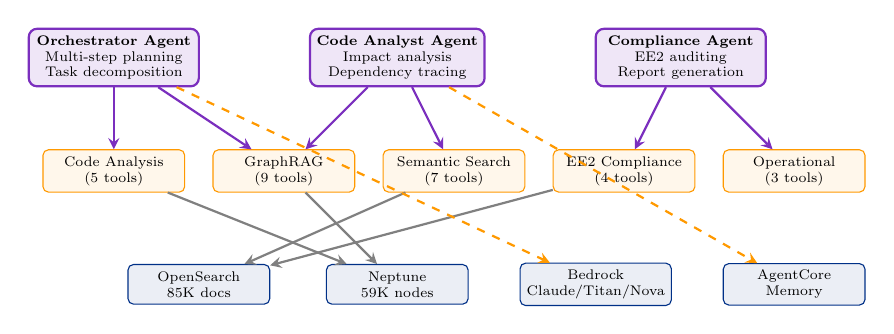
\begin{tikzpicture}[
    scale=0.72,
    every node/.style={transform shape},
    agent/.style={rectangle, draw=strandspurple, fill=strandspurple!12,
                 minimum width=3cm, minimum height=0.9cm, font=\scriptsize,
                 align=center, rounded corners=3pt, thick},
    tool/.style={rectangle, draw=awsorange, fill=awsorange!8,
                minimum width=2.5cm, minimum height=0.7cm, font=\scriptsize,
                align=center, rounded corners=2pt},
    infra/.style={rectangle, draw=noaablue, fill=noaablue!8,
                 minimum width=2.5cm, minimum height=0.7cm, font=\scriptsize,
                 align=center, rounded corners=2pt},
    arrow/.style={->, thick, >=stealth}
]

% Agents layer
\node[agent] at (0,5) (orchestrator) {\textbf{Orchestrator Agent}\\Multi-step planning\\Task decomposition};
\node[agent] at (5,5) (analyst) {\textbf{Code Analyst Agent}\\Impact analysis\\Dependency tracing};
\node[agent] at (10,5) (compliance) {\textbf{Compliance Agent}\\EE2 auditing\\Report generation};

% Tools layer
\node[tool] at (0,3) (code-tools) {Code Analysis\\(5 tools)};
\node[tool] at (3,3) (graph-tools) {GraphRAG\\(9 tools)};
\node[tool] at (6,3) (search-tools) {Semantic Search\\(7 tools)};
\node[tool] at (9,3) (ee2-tools) {EE2 Compliance\\(4 tools)};
\node[tool] at (12,3) (ops-tools) {Operational\\(3 tools)};

% Infrastructure
\node[infra] at (1.5,1) (opensearch) {OpenSearch\\85K docs};
\node[infra] at (5,1) (neptune) {Neptune\\59K nodes};
\node[infra] at (8.5,1) (bedrock) {Bedrock\\Claude/Titan/Nova};
\node[infra] at (12,1) (memory) {AgentCore\\Memory};

% Arrows
\draw[arrow, strandspurple] (orchestrator) -- (code-tools);
\draw[arrow, strandspurple] (orchestrator) -- (graph-tools);
\draw[arrow, strandspurple] (analyst) -- (graph-tools);
\draw[arrow, strandspurple] (analyst) -- (search-tools);
\draw[arrow, strandspurple] (compliance) -- (ee2-tools);
\draw[arrow, strandspurple] (compliance) -- (ops-tools);

\draw[arrow, gray] (code-tools) -- (neptune);
\draw[arrow, gray] (graph-tools) -- (neptune);
\draw[arrow, gray] (search-tools) -- (opensearch);
\draw[arrow, gray] (ee2-tools) -- (opensearch);

\draw[arrow, awsorange, dashed] (orchestrator) -- (bedrock);
\draw[arrow, awsorange, dashed] (analyst) -- (memory);

\end{tikzpicture}
\caption{Path B vision: Strands agents orchestrating MCP tools with Bedrock
models and AgentCore Memory.}
\label{fig:path-b-vision}
\end{figure}

\subsection{Strands Agents SDK Capabilities}

The Strands Agents SDK (open-source, Python) provides:

\begin{itemize}[noitemsep]
    \item \textbf{Model-driven agents}: Define agent behavior in a few lines;
          the LLM decides which tools to call and in what order
    \item \textbf{Multi-agent orchestration}: GraphBuilder for directed
          workflows, handoffs between specialized agents, swarm patterns
    \item \textbf{Tool integration}: Native MCP tool consumption---our 51
          tools become first-class Strands tools
    \item \textbf{Memory integration}: Built-in session manager with
          AgentCore Memory for STM and LTM
    \item \textbf{Model agnostic}: Works with Bedrock (Claude, Nova, Titan),
          OpenAI, or any LLM provider
    \item \textbf{Observability}: OpenTelemetry instrumentation built-in
\end{itemize}

\subsection{Example: Autonomous Impact Analysis Agent}

\begin{lstlisting}[language=Python,caption={Strands agent that autonomously analyzes code change impact.}]
from strands import Agent
from strands.tools.mcp import MCPClient

# Connect to our MCP server (all 51 tools available)
mcp = MCPClient("http://localhost:8000/mcp")

# Create an agent with access to our tools
analyst = Agent(
    model="us.anthropic.claude-opus-4-6-v1:0",
    tools=mcp.list_tools(),
    system_prompt="""You are a code impact analyst for the NOAA
    Global Forecast System. When asked about a code change:
    1. Use get_code_context to understand the symbol
    2. Use get_change_impact to assess blast radius
    3. Use trace_full_execution_chain to find affected workflows
    4. Use search_documentation for relevant docs
    5. Produce a structured impact report."""
)

# The agent autonomously calls tools and reasons
result = analyst("Analyze the impact of changing setuprad")
\end{lstlisting}

\subsection{Port Strategy: Module-by-Module}

The port does not need to be all-or-nothing. Python and Node.js can
coexist during the transition:

\begin{table}[H]
\centering
\footnotesize
\begin{tabular}{@{}llll@{}}
\toprule
\textbf{Phase} & \textbf{Module} & \textbf{Effort} & \textbf{Rationale} \\
\midrule
B1 & FastMCP wrapper + tool registration & 1 week & Scaffolding \\
B2 & OpenSearch adapter (Python) & 1 week & Already have \texttt{aws\_backend.py} \\
B3 & Neptune adapter (Python) & 2 weeks & openCypher via \texttt{neo4j} driver \\
B4 & SemanticSearchTools & 1 week & Vector queries \\
B5 & CodeAnalysisTools & 2 weeks & Graph traversal \\
B6 & GraphRAGTools + GGSR & 3 weeks & Most complex module \\
B7 & EE2ComplianceTools & 1 week & Pattern matching \\
B8 & OperationalTools & 1 week & Hybrid queries \\
B9 & SDDWorkflowTools & 1 week & File I/O \\
B10 & WorkflowInfoTools & 3 days & Static tools \\
B11 & Strands agent layer & 2 weeks & Multi-agent orchestration \\
B12 & AgentCore Memory integration & 1 week & STM + LTM \\
B13 & AgentCore Gateway + Policy & 1 week & Cedar policies \\
B14 & Observability + Evaluations & 1 week & OpenTelemetry \\
\midrule
& \textbf{Total} & \textbf{$\sim$16 weeks} & \\
\bottomrule
\end{tabular}
\caption{Module-by-module port schedule.}
\end{table}

\subsection{What Already Exists in Python}

The ingestion pipeline is already Python ($\sim$4,000 lines):

\begin{itemize}[noitemsep]
    \item \texttt{embedding\_registry.py} --- Model profiles and registry
    \item \texttt{embedding\_provider.py} --- Local and Bedrock providers
    \item \texttt{ingestion\_base.py} --- BaseIngester with backend routing
    \item \texttt{aws\_backend.py} --- OpenSearch and Neptune clients
    \item \texttt{benchmark\_runner.py} --- Quality metrics
    \item \texttt{drift\_detector.py} --- Embedding drift detection
    \item \texttt{fine\_tuning\_pipeline.py} --- SageMaker training
    \item \texttt{hard\_negative\_miner.py} --- Graph-powered training data
    \item 7 ingestion scripts (code, docs, Fortran, shell, jjobs, etc.)
\end{itemize}

These provide a foundation---the OpenSearch and Neptune client code can
be reused directly in the Python MCP server.

%===============================================================================
\section{New Capabilities Unlocked by Path B}
%===============================================================================

\subsection{Autonomous Multi-Agent Workflows}

With Strands Agents, we can build specialized agents that collaborate:

\begin{table}[H]
\centering
\footnotesize
\begin{tabular}{@{}p{3cm}p{4cm}p{6cm}@{}}
\toprule
\textbf{Agent} & \textbf{Tools Used} & \textbf{Autonomous Behavior} \\
\midrule
Code Analyst & \texttt{get\_code\_context}, \texttt{get\_change\_impact}, \texttt{trace\_full\_execution\_chain} & Produces impact reports for PRs without human prompting \\
Compliance Auditor & \texttt{scan\_repository\_compliance}, \texttt{analyze\_ee2\_compliance} & Runs nightly EE2 audits, files issues for violations \\
Knowledge Curator & \texttt{check\_knowledge\_integrity}, \texttt{drift\_detector} & Detects stale embeddings, triggers re-ingestion \\
Documentation Crawler & AgentCore Browser & Crawls rate-limited sites with retry, handles JS rendering \\
Benchmark Runner & AgentCore Code Interpreter & Runs quality benchmarks on schedule, alerts on regression \\
\bottomrule
\end{tabular}
\caption{Specialized agents enabled by Strands + AgentCore.}
\end{table}

\subsection{Persistent Cross-Session Memory}

AgentCore Memory enables agents to learn from past interactions:

\begin{itemize}[noitemsep]
    \item \textbf{Short-term}: Conversation context within a Kiro session
          (replaces our stateless HTTP transport)
    \item \textbf{Long-term}: ``User frequently asks about JGLOBAL\_FORECAST
          and setuprad''---agent pre-loads relevant context
    \item \textbf{Shared}: Multiple agents share a memory store---the
          Compliance Auditor's findings are available to the Code Analyst
    \item \textbf{SDD sessions}: Development session state persists in
          managed memory instead of \texttt{history.jsonl}
\end{itemize}

\subsection{Bedrock Foundation Model Integration}

A Python port enables direct Bedrock API integration:

\begin{itemize}[noitemsep]
    \item \textbf{Claude Opus 4.6/4.7} for complex reasoning about code
          architecture
    \item \textbf{Claude Sonnet 4.6} for fast tool-calling in multi-step
          workflows
    \item \textbf{Claude Haiku 4.5} for high-volume, low-cost operations
          (e.g., batch compliance checking)
    \item \textbf{Amazon Nova} for cost-effective embedding generation
    \item \textbf{Model routing}: Strands can route to different models
          based on task complexity
\end{itemize}

\subsection{Cedar Policy Enforcement}

Fine-grained, deterministic access control:

\begin{itemize}[noitemsep]
    \item Per-tool permissions (e.g., only auditors can run compliance scans)
    \item Per-user rate limiting (e.g., 100 tool calls/hour for external users)
    \item Data-level restrictions (e.g., restrict \texttt{search\_documentation}
          to specific collections)
    \item Audit trail of every policy decision
\end{itemize}

\subsection{Production Observability}

Replace custom health monitoring with managed infrastructure:

\begin{itemize}[noitemsep]
    \item OpenTelemetry traces for every tool call (latency, errors, tokens)
    \item CloudWatch dashboards with per-tool metrics
    \item Automatic anomaly detection (replaces \texttt{get\_health\_trend})
    \item Integration with Dynatrace, Elastic, or Datadog
\end{itemize}

%===============================================================================
\section{Risk Assessment}
%===============================================================================

\begin{table}[H]
\centering
\footnotesize
\begin{tabular}{@{}p{3.5cm}p{2cm}p{2cm}p{5.5cm}@{}}
\toprule
\textbf{Risk} & \textbf{Likelihood} & \textbf{Impact} & \textbf{Mitigation} \\
\midrule
Python port introduces bugs & Medium & High & Module-by-module port with parity tests against Node.js baseline \\
Neptune openCypher differences resurface & Low & Medium & Already solved---port the fixes, not the bugs \\
AgentCore service limits & Low & Medium & Start with Runtime, add services incrementally \\
Strands SDK breaking changes & Low & Low & Pin SDK version, test on upgrade \\
Team Python proficiency & Low & Low & Ingestion pipeline already Python; team is bilingual \\
Port takes longer than estimated & Medium & Medium & Node.js server continues serving production during port \\
\bottomrule
\end{tabular}
\caption{Risk assessment for Path B.}
\end{table}

%===============================================================================
\section{Quarterly Roadmap}
%===============================================================================

\begin{table}[H]
\centering
\footnotesize
\begin{tabular}{@{}p{2cm}p{4cm}p{7cm}@{}}
\toprule
\textbf{Quarter} & \textbf{Milestone} & \textbf{Deliverables} \\
\midrule
\textbf{Q3 2026} & Path A: Container Deploy & AgentCore Runtime deployment, Cognito auth, remove dev bridge. Node.js server in production. \\
\midrule
\textbf{Q4 2026} & Path B Phase 1: Foundation & Python FastMCP server with OpenSearch + Neptune adapters. First 20 tools ported. Parity tests passing. Node.js still serving production. \\
\midrule
\textbf{Q1 2027} & Path B Phase 2: Full Port & All 51 tools in Python. GGSR ported. Strands agent layer. AgentCore Memory + Gateway + Policy. Cutover from Node.js. \\
\midrule
\textbf{Q2 2027} & Path B Phase 3: Agents & Multi-agent orchestration. Autonomous compliance auditor. Knowledge curator. Browser-based documentation crawler. Full observability. \\
\bottomrule
\end{tabular}
\caption{Quarterly roadmap for AgentCore adoption.}
\end{table}

%===============================================================================
\section{Cost Considerations}
%===============================================================================

AgentCore uses consumption-based pricing with no upfront commitments:

\begin{itemize}[noitemsep]
    \item \textbf{Runtime}: Per-second billing for container execution time
    \item \textbf{Memory}: Per-GB-month for stored memory + per-request for
          retrieval
    \item \textbf{Gateway}: Per-request for tool invocations
    \item \textbf{Observability}: Standard CloudWatch pricing for traces/logs
    \item \textbf{Bedrock models}: Per-token pricing (varies by model)
\end{itemize}

Current cost baseline: EC2 instance (\$0.10/hr) + Neptune (\$0.35/hr) +
OpenSearch (\$0.24/hr) $\approx$ \$500/month. AgentCore Runtime would
replace the EC2 cost with per-invocation pricing, potentially reducing
costs during low-usage periods.

%===============================================================================
\section{Conclusion and Recommendation}
%===============================================================================

The MDC MCP/RAG platform stands at an architectural inflection point.
Path~A (container deployment) is a tactical win that delivers production
readiness in 1--2 weeks. Path~B (full Python port) is a strategic
investment that transforms the platform from a tool server into an
autonomous agent ecosystem with persistent memory, policy enforcement,
observability, and multi-agent orchestration.

\textbf{Recommendation}: Execute both paths sequentially.

\begin{enumerate}[noitemsep]
    \item \textbf{Q3 2026}: Deploy Node.js server to AgentCore Runtime
          (Path~A). Ship it.
    \item \textbf{Q4 2026}: Begin Python port, module by module, with
          parity tests against the Node.js baseline.
    \item \textbf{Q1 2027}: Complete port, activate AgentCore Memory +
          Gateway + Policy. Cutover.
    \item \textbf{Q2 2027}: Build autonomous agents. Compliance auditor.
          Knowledge curator. Full observability.
\end{enumerate}

The Node.js server continues serving production traffic throughout the
port. No downtime. No big-bang migration. Each module is validated
against the existing baseline before cutover.

The question is not whether to adopt AgentCore---it is how fast to move
from tactical deployment to strategic transformation.

%===============================================================================
\section*{References}
%===============================================================================

\begin{enumerate}[noitemsep]
    \item AWS. ``Amazon Bedrock AgentCore.''
          \url{https://docs.aws.amazon.com/bedrock-agentcore/latest/devguide/what-is-bedrock-agentcore.html}, 2025.
    \item AWS. ``Deploy MCP servers in AgentCore Runtime.''
          \url{https://docs.aws.amazon.com/bedrock-agentcore/latest/devguide/runtime-mcp.html}, 2025.
    \item AWS. ``Strands Agents 1.0: Production-Ready Multi-Agent Orchestration.''
          \url{https://aws.amazon.com/blogs/opensource/introducing-strands-agents-1-0-production-ready-multi-agent-orchestration-made-simple}, 2025.
    \item AWS. ``AgentCore Memory: Building Context-Aware Agents.''
          \url{https://aws.amazon.com/blogs/machine-learning/amazon-bedrock-agentcore-memory-building-context-aware-agents/}, 2025.
    \item AWS. ``Secure AI Agents with Policy in AgentCore.''
          \url{https://aws.amazon.com/blogs/machine-learning/secure-ai-agents-with-policy-in-amazon-bedrock-agentcore/}, 2025.
    \item AWS. ``Transform MCP Architecture: Unite MCP Servers through AgentCore Gateway.''
          \url{https://aws.amazon.com/blogs/machine-learning/transform-your-mcp-architecture-unite-mcp-servers-through-agentcore-gateway/}, 2025.
    \item AWS. ``Customize Agent Workflows with Advanced Orchestration using Strands Agents.''
          \url{https://aws.amazon.com/blogs/machine-learning/customize-agent-workflows-with-advanced-orchestration-techniques-using-strands-agents/}, 2025.
    \item Strands Agents SDK. \url{https://github.com/strands-agents/sdk-python}, 2025.
    \item Cedar Policy Language. \url{https://www.cedarpolicy.com/}, AWS, 2023.
    \item Anthropic. ``Model Context Protocol Specification.''
          \url{https://spec.modelcontextprotocol.io/}, 2024.
\end{enumerate}

\end{document}
